\documentclass[12pt,titlepage,oneside]{book}
%------------------------------Package Includes in alphabetical order
\usepackage{adjustbox} %Allows for the creation of boxes that can be sized independently
\usepackage{amsmath, amssymb, amsthm}% For mathematical Symbols
\usepackage{fancyhdr} % Puts headers and footers into the document
\usepackage{feynmp, feynmp-auto} % Allows for use of Feynmann diagram environments
\usepackage[font={small,it}]{caption} %Allows for small captions with an italicised font
\usepackage{gensymb} %For use of \degree.
\usepackage[top=2.5cm, bottom=1.8cm,left=4.0cm,right=1.5cm]{geometry} % Alters the margins. % These margins are the university guidelines
\usepackage{graphicx} % Standard package for importing graphics files
\usepackage[hidelinks]{hyperref} % All refernces will jump to place they are declared. Hyperrefs will be the color of the text.
\usepackage{lineno} % For line numbers when i'm writing drafts
\usepackage[version=4]{mhchem} % Allows correct index notation for chemical elements
\usepackage{setspace}  % [onehalfspacing] gives one-and-a-half line spacing. Doublespacing is another option and can be changed in the text (\doublespacing)
\usepackage{rotating} % Allows the addition of sideways figures, caption included.
\usepackage{subfig} % Allows for manipulation of sub-figures. Cannot be used in conjection with subcaption package.
\usepackage[table,xcdraw]{xcolor}  %Allows for table edition flexibility and usage of certain colours.
\usepackage{tabu} %Allows for greater table edition flexibility.
\usepackage[toc,page]{appendix}% for the appendices.
\usepackage{xcolor}

%-------------------------------Stylistic Choices
\newcommand{\tcr}[1]{\textcolor{red}{#1}} % Note to self
\newcommand{\tcg}[1]{\textcolor{green}{#1}} % To be moved to a different section
\newcommand{\tcc}[1]{\textcolor{cyan}{#1}} % Things to expand upon

\newcommand{\tit}[1]{\textit{#1}} % Emphasise new variables.

%Things I am sick to death of writing all the time.
\newcommand{\MC}{MC simulations }
\newcommand{\MCed}{MC simulated events }                                               
\newcommand{\W}{W-boson }                                                    
\newcommand{\Z}{Z-boson }  
\newcommand{\Ra}{Resolved analysis }
\newcommand{\Ba}{Boosted analysis }  
\newcommand{\SM}{Standard Model } 

%greek letters
\newcommand{\etam}{$\eta$ }
\newcommand{\phim}{$\phi$ }
\newcommand{\num}{$\nu$ }
\newcommand{\mum}{$\mu$ }
\newcommand{\sigmam}{$\sigma$ }
\newcommand{\thetam}{$\theta$ }
\newcommand{\chisquared}{$\chi^2$ }

%The same thing as above but with no space after it
\newcommand{\mc}{MC simulations} 
\newcommand{\mced}{MC simulated events}
\newcommand{\w}{W-boson}                                                   
\newcommand{\z}{Z-boson}                                                    
\newcommand{\ra}{Resolved analysis}
\newcommand{\ba}{Boosted analysis}  
\newcommand{\sm}{Standard Model} 

\newcommand{\etamo}{$\eta$}
\newcommand{\phimo}{$\phi$}
\newcommand{\numo}{$\nu$}
\newcommand{\mumo}{$\mu$}
\newcommand{\sigmamo}{$\sigma$}
\newcommand{\thetamo}{$\theta$}
\newcommand{\chisquaredo}{$\chi^2$}


%Variable definitions 
\newcommand{\dn}{\ensuremath{d_0} }                                    %Transverse impact parameter d_0.           
	\newcommand{\dno}{\ensuremath{d_0}}                                     %Transverse impact parameter d_0 at the end of a phrase or sentence.      
\newcommand{\pt}{\ensuremath{p_{\text{T}}} }
\newcommand{\ptv}{\ensuremath{p_{\text{T}}^{V}} }                      %Vector boson transverse momentum 
	\newcommand{\ptvo}{\ensuremath{p_{\text{T}}^{V}} }                      %Vector boson transverse momentum at the end of a phrase or sentence.
\newcommand{\ptz}{\ensuremath{p_{\text{T}}^{Z}} }                      %Z boson transverse momentum 
\newcommand{\ptw}{\ensuremath{p_{\text{T}}^{W}} }                      %W boson transverse momentum 
\newcommand{\met}{\ensuremath{E_{\text{T}}^{\text{miss}}} }            %missing transverse energy 
	\newcommand{\meto}{\ensuremath{E_{\text{T}}^{\text{miss}}}}             %missing transverse energy at the end of a phrase or sentence.
\newcommand{\mpt}{\ensuremath{E_{\text{T,~trk}}^{\text{miss}}} }       %track-based missing transverse energy 
\newcommand{\mJ}{\ensuremath{m_{\text{J}}} }                           %large-R jet  mass 
\newcommand{\mll}{\ensuremath{m_{ll}} }                                %di-lepton  mass 
\newcommand{\gev}{\ensuremath{~GeV }}								 %Units of energy
	\newcommand{\gevo}{\ensuremath{~GeV}}								  %Units of energy at the end og a phrase or sentence
	
%Analyses and Regions
\newcommand{\Hbb}{\ensuremath{H \to b\bar{b}} }                        %Hbb
\newcommand{\VHbb}{\ensuremath{VH, H\to b\bar{b}} }                    %VHbb
\newcommand{\ttbar}{\ensuremath{t\bar{t}} }                            %ttbar

\newcommand{\medPTV}{\ensuremath{75~GeV \leq \ptv < 150~GeV} }           %medium PTV region
\newcommand{\highPTV}{\ensuremath{150~GeV \leq \ptv < 250~GeV} }         %high PTV region
\newcommand{\extremePTV}{\ensuremath{\ptv \ge 250~GeV} }                 %extreme PTV region
\newcommand{\immensePTV}{\ensuremath{250~GeV \leq \ptv  < 400~GeV} }         %immense PTV region
\newcommand{\utmostPTV}{\ensuremath{\ptv \ge 400~GeV} }                      %utmost PTV region

% VHbb channels                                                                                                                            
\newcommand{\zlep}{\ensuremath{0}-lepton }
\newcommand{\olep}{\ensuremath{1}-lepton }
\newcommand{\tlep}{\ensuremath{2}-lepton }

% Other useful shortcuts
\newcommand{\ifb}{fb\ensuremath{^{-1}} }                               % integrated luminosity
\newcommand{\lumi}{\ensuremath{139} fb\ensuremath{^{-1}} }             % physics integrated luminosity at ATLAS
\newcommand{\sorb}{\ensuremath{\frac{s}{\sqrt{b}}} }                   % signal over root background
\newcommand{\abs}[1]{\ensuremath{\mid #1\mid} }                        % for absolute value of something
\newcommand{\range}[3]{\ensuremath{#2 < #1 < #3} }                     % [1] between range of [2] and [3] exclusive
\newcommand{\rangei}[3]{\ensuremath{#2 \leq #1 \leq #3} }              % [1] between range of [2] and [3] inclusive

\setlength{\parindent}{0pt} % No indents
\begin{document}% Starts the Document
%--------------------------------------------------------------------------------TITLE PAGE
	\begin{center} %Centres the items that follow
	
\includegraphics[width=0.7\textwidth]{ExperPartPhys_colour.pdf}~\\[4mm]%Inserts University Logo
	School of Physics and Astronomy\\
	University of Glasgow\\
	Glasgow\\
	G12 8QQ\\[4mm] %Adds the postcode of the uni and then a 4mm gap.

	\rule[0.4cm]{15cm}{.2pt}\\ %Adds a line underneath 

	{\Huge \textbf{VHbb: A Story \\ \tcr{NOTHING TO SEE HERE}}}
	\rule[0.4cm]{15cm}{.2pt}\\ %Adds a line underneath 
	{\Huge A Study of The Associated Production of the Higgs Boson with a Vector Boson with the Run II dataset from the ATLAS experiment at CERN.\\[1cm] Fake Rate Studies}\\[2cm] %Title
	{\LARGE Dwayne Isaac Patrick Laurence \textsc{Spiteri}}\\[1cm] %Author
	{\small \today}\\[1cm] %Date
	{\small 
		Submitted in fulfilment of the requirements for the\\
		Degree of Doctor of Philosophy}\\[1cm] %Word Count
	\rule[0.4cm]{15cm}{.2pt} 
	\end{center}


\frontmatter  % Turn off chapter numbering, use roman page numbers

\chapter{Abstract}
	\noindent {\small This thesis describes the main body of work conducted in the ATLAS experiment, including, my work in physics analysis of \VHbb and my work in Fake rates for Tracking CP.}


\chapter{Acknowledgements}
\doublespacing


\chapter{Declaration}
I do declare that this is all my own work. Except the parts that I ... \\ Plagiarised, let no-one else's work evade your eyes. Remember why the good Lord made your eyes, so don't shade your eyes but plagiarise, plagiarise, plagiarise only be sure to always call it please: `research' - Tom Lehrer

\singlespacing

\phantomsection
\tableofcontents
\cleardoublepage

\phantomsection
\addcontentsline{toc}{chapter}{List of Figures}
\listoffigures
\cleardoublepage

\phantomsection
\addcontentsline{toc}{chapter}{List of Tables}
\listoftables

\doublespacing

\mainmatter % Turn on chapter numbering, reset page numbers, use arabic
\linenumbers % To be commented out in the final draft.

\chapter{Introduction}
\label{chap:intro}
%----------------------------------------------------------------- INTRODUCTION
\section{Opening Remarks}
\initial{A}utumn is the season. It is a dry September afternoon and you find yourself on a train. Temporarily setting aside your book, your phone, or your laptop, your attention turns to the picturesque countryside that streams past.  What do you see? \\

Do you see the solar photons undergoing Rayleigh scattering in the upper atmosphere to make the sky appear blue\footnote{The sun gives off lower intensities of violet light than blue light; this coupled with the fact that our eyes are more sensitive to blue light than violet light meaning that we see the sky as blue.}? Or the refraction of that light in water droplets to produce a rainbow? Do you look at the trunks of the trees racing by and wonder exactly how you see a brown colour as there was no brown in the rainbow you have just seen\footnote{Colour is made from three components: hue, brightness, and saturation. Brown is just an orange that does not reflect much light back to your eyes.}? Do you see the birds flying past as being in an eternal battle with the forces of gravity, air resistance and upthrust keeping them aloft, all the while oblivious to the billions of neutrinos passing through them? Chances are while, like myself, you are a massive nerd because you are reading this, you do not see the world in this way (unless, of course, you are under the influence of some sort of narcotics). But \textbf{Physics}$^{\text{TM}}$ is the science of trying to describe how the natural world works and the properties of matter and energy. Particle physics attempts to do this by deconstructing the universe (and by extension, the world) into a set of fundamental building blocks with rules that govern their interactions. This is referred to as a model. Currently the best model that is consistent with two centuries of experimental data, is a set of quantum field theories known as the Standard Model.

%----------------------------------------------------------------- BACKGROUND
\section{The Forces of Nature}
A \tit{force} is the name given to any interaction that changes the motion of an object if not equally opposed by another force. Physics asserts that every force in nature that acts on a body is reducible to one of four fundamental forces. Two forces govern long-range interactions between objects: electromagnetism and gravity; and two forces are only relevant on atomic-scales: the weak and strong forces.\\

The strong force is the strongest of these forces and is responsible for holding atomic nuclei together despite the fact the constituent protons all have the same sign electric charge and therefore repel each other. The electromagnetic force is the next strongest force and governs the interactions between particles that are electrically charged. The weak force is responsible for radioactive decay and is the main process of nuclear fusion in stars. The last force is gravity, the only force relevant across the large distances of the cosmos, but by far the weakest at the atomic scale (see Table \ref{tab:relForceStr} below). Gravity is an attractive force that acts between all objects that have mass.\\

\begin{table}[h!]
\centering
\caption[Table showing the strength of all the fundamental forces relative to the strongest force; the strong force.]{A table showing the strength of all the fundamental forces relative to the strongest force: the strong force~\cite{Forces}. The force-distances mentioned here are governed by the lifetime of the particles that mediate the forces. Since these relative strengths are energy dependent, these values are approximations made at ~200\,MeV.}
\label{tab:relForceStr}
\begin{tabular}{|l|l|l|}
\hline
\textbf{Force} & \textbf{Relative strength} & \textbf{Range ($10^{-15}$\,m)} \\ \hline
\textbf{Strong} & $1$ & $\sim 1$ \\ \hline
\textbf{Electromagnetic} & $\sim 1/137$ & $\infty$ \\ \hline
\textbf{Weak force} & $\sim 10^{-6}$ & $\sim 10^{-3}$~\cite{Zboson}\\ \hline
\textbf{Gravitational} & $\sim 10^{-39}$ & $\infty$ \\ \hline
\end{tabular}
\end{table}

These four forces are conservative, which means the relative strength of these forces is only dependent on the distance between two objects that can undergo the same interaction. A description that permeates all of space able to describe the way these forces propagate and interact with objects is called a `field', and it allows us to come up with a mathematical formalism to describe these forces. For sub-atomic particles that experience the fundamental forces, in order to accurately depict their behaviour, a single model interweaving these forces and the fundamental particles that interact via them is required. This mathematical description is the Standard Model.
 
\section{The Standard Model}
The Standard Model (SM) describes the observable universe on a sub-atomic level by the interactions of fundamental particles.\\

There are twelve \tit{fermionic} or `matter' particles: six quarks that interact via the strong, electromagnetic and weak forces; three electrically charged leptons that interact with the electromagnetic and weak forces; and three electrically neutral leptons called neutrinos that interact only with the weak force. These twelve particles also have distinct anti-particles. Anti-matter particles, however, are seen as trivial extensions of matter particles and are thus not depicted as individually separate from their matter counterparts in the Standard Model\footnote{An anti-particle has the same mass as its particle counterpart, but all its quantum numbers are reversed. For example the up quark has a unit of colour charge [red, blue, green] and a electric charge relative to the charge of an electron of $\frac{2}{3}$, and its antiparticle counterpart (the anti-up quark) has a unit of anti-colour charge [anti-red, anti-blue, anti-green] and an relative electric charge of $-\frac{2}{3}$.}. These matter particles can combine in many different ways to create other particles.\\

\begin{sidewaysfigure}[thbp!]
	\centering
	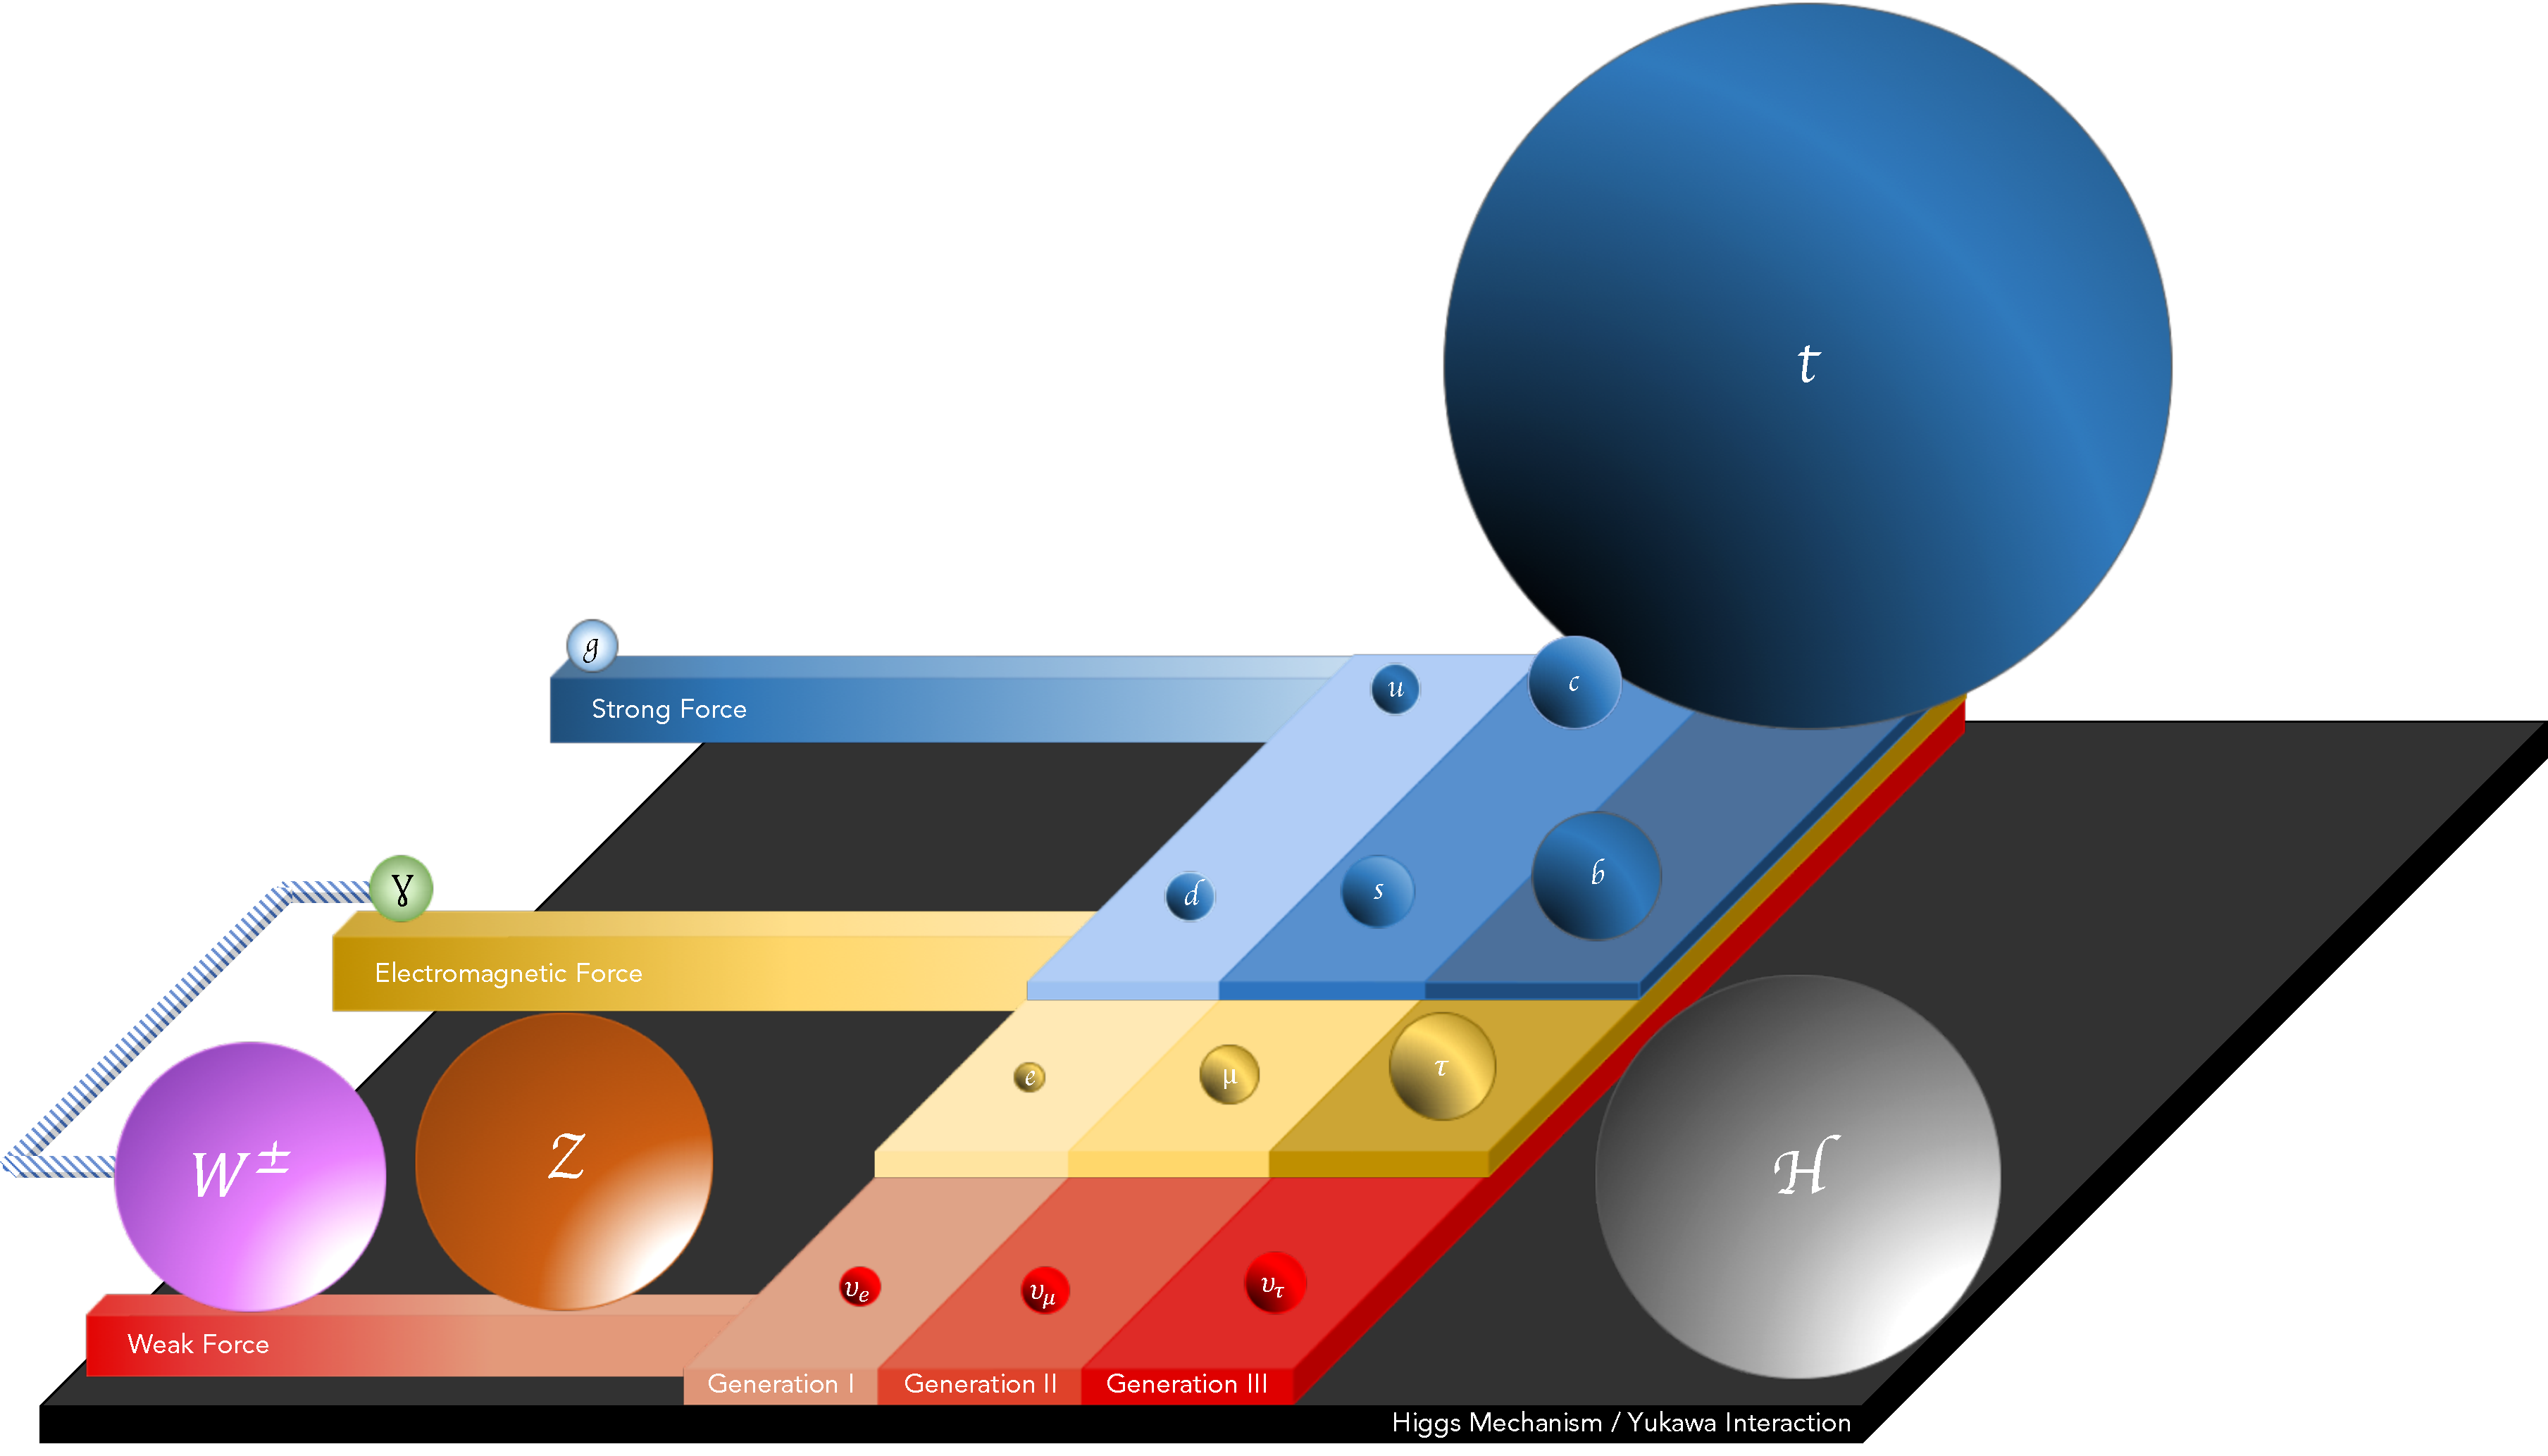
\includegraphics[width=0.90\textwidth]{Introduction/SM.pdf}
	\caption[Depiction of the \SM showing its seventeen particles (five bosons and twelve fermions), as spheres on plinths that represent the fundamental forces.]{\footnotesize{Depiction of the \sm. There are seventeen particles, antiparticles notwithstanding, shown as spheres consisting of five bosons and twelve fermions. The particles known as fermions are all on the central plinth. Quarks are depicted in blue, charged leptons in yellow/gold and the neutrinos in red. The quarks are separated into two rows; the top row has a fundamental electric charge of $\frac{2}{3}$ while the bottom has a fundamental electric charge of $-\frac{1}{3}$. The force-carrying bosons have interactions with all particles of the colour of the bars that come off the central plinth. All particles on plinths have interactions with all other particles on all levels higher than it, i.e. the gluon will interact only with the quarks but the photon will interact with both the quarks and the charged leptons but not the gluon. The exception to this is the \W as it has electromagnetic charge, so can interact with a photon. The fermion plinth is divided into three groups of particles called generations. Between each generation all the quantum numbers barring flavour are the same but the higher the generation number the more massive the rest mass of the particles. All particles in white text are massive, and the sizes of the spheres are indicators of the relative masses of the particles with the exception of the electron and neutrinos which would be too small so have been scaled up. All particles in black text are massless. The Higgs particle interacts with all massive particles. If the white-gradient shading on the ball is to the bottom right then these particles interact with the Higgs via the Higgs Mechanism, and if the black-gradient shading on the particle ball is to the bottom left then the interactions with the Higgs are via the Yukawa interaction.}}
	\label{fig:SM} 
\end{sidewaysfigure}

There are four force-carrying \tit{gauge bosons} that interact with particles to mediate the fundamental forces: the gluon, which mediates the strong force; the photon, which mediates the electromagnetic force; and two weak bosons, the \W and the \Z which mediate the weak force. Since the \W has electric charge, two \w s exist: the $W^+$ and the $W^-$, but they are anti-particles of each other. The gluon (and quarks also) carry colour change, so technically all possible colours that the particles can have count as separate particles, but again this `colour index' is a trivial extension of the number of particles and are thus discounted. \\

The last particle in the \SM description is the Higgs boson. The Higgs boson is a physical manifestation of the Higgs field. Particles that interact with this Higgs field gain their `rest' mass. A pictorial depiction of the particles in the \SM is shown in Figure \ref{fig:SM}.\\

This means that there are seventeen fundamental particles, and of these, the Higgs particle, discovered only in July of 2012 by the ATLAS (A Toroidal LHC ApparatuS) \cite{ATLASHiggsDisc} and CMS (Compact Muon Solenoid) \cite{CMSHiggsDisc} experiments, is the least well known in terms of its characteristics. This PhD thesis will describe my contributions to increasing our understanding of the Higgs boson, and specifically the  discovery of the decay mode of a Higgs particle into a bottom and anti-bottom quark (\Hbb).\\

The astute readers among you (who didn't already know) will have spotted one of the failings of the \SM in this brief description. It has no mechanism through which particles interact gravitationally with each other. While a gravitational attraction between particles is expected to be extremely weak, such a mechanism is possible. However, there are both experimental and theoretical challenges in uniting gravity with the \sm. From a theoretical point of view in constructing the \sm, it has not proved possible thus far to weave Einstein's General Relativity into the \sm. In addition, experimentally, the particle that would be responsible for mediating the interaction, the graviton ($g^0$), has not been detected.\\

The field of particle physics is ever-evolving and minor alterations are made to the \SM `particle zoo' all the time such as the addition of newly discovered particles and the recording of properties to greater precisions~\cite{PDG2018Booklet,PDG2016Booklet,PDG2014Booklet,PDG2012Booklet,
PDG2010Booklet,PDG2008Booklet,PDG2006Booklet,PDG2002Booklet,
PDG2000Booklet,PDG1998Booklet,PDG1994Booklet}. These are regularly done and one such way of communicating these changes are the Particle Data Group Booklets , some of which are present in Figure \ref{fig:booklets}. The first step on this journey is a step into the theoretical side to ask why the Standard Model needs a Higgs Boson.
\begin{figure}[htbp]
	\centering
	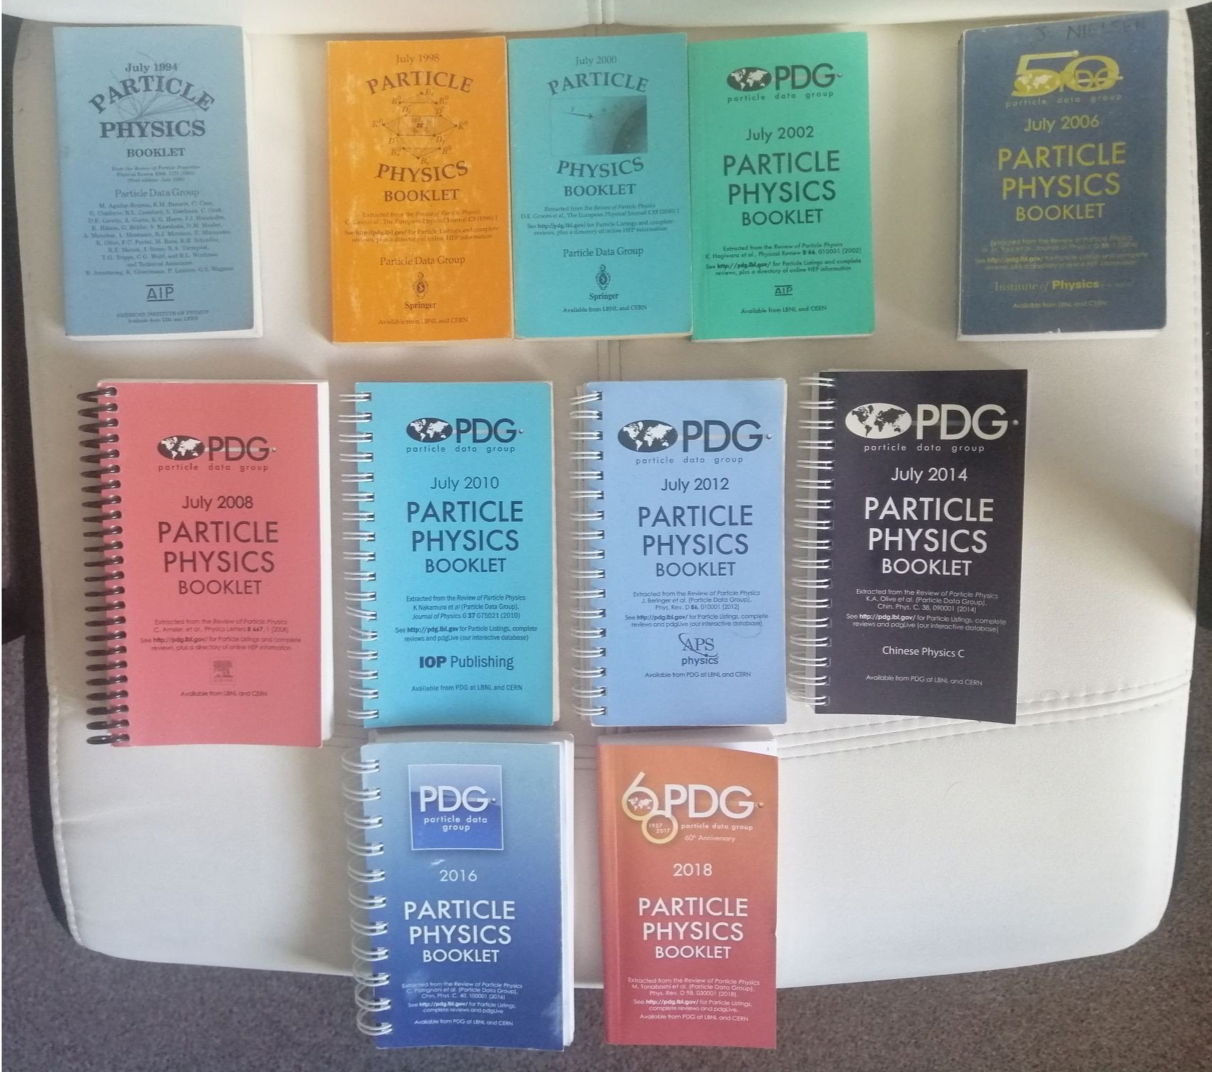
\includegraphics[width=0.75\textwidth]{Introduction/PDGs.png}
	\caption[The particle data booklets that I currently own.]{The particle data booklets that I currently own starting from the year I was born. If you have physical copies of the 1996 or 2004 versions lying around, I would be interested in taking them off your hands.}
	\label{fig:booklets}
\end{figure}

\chapter{Standard Model Theory}
\label{chap:theory}
\input{Theory/Theory.tex}

\chapter{CERN and The LHC}
\label{chap:CERNLHC}
\input{LHC/LHC.tex}

\chapter{The ATLAS Detector}
\label{chap:ATLAS}
\input{ATLAS/ATLAS.tex}

\chapter{Fake Tracks in the ATLAS Detector}
\label{chap:FakeTracks}
\input{FakeTracks/FakeTracks.tex}

\chapter{Object Selection}
\label{chap:ObjSel}
\input{ObjectSelection/ObjectSelection.tex}

\chapter{An overview of the VHbb Analyses}
\label{chap:Analyses}
\input{TheAnalyses/TheAnalyses.tex}

\chapter{Statistics, Fits and Significances}
\label{chap:Statfits}
\input{StatFits/StatFits.tex}

\chapter{\met Triggers in the \tlep Analyses} % Bold the mathematics as well.
\label{chap:METTriggerStudy}
\input{TriggerStudy/TriggerStudy.tex}

\chapter{Conclusion}
\label{chap:conc}
\input{Conclusion/Conclusion.tex}

\begin{appendices}
\chapter{Impact of \tlep Significance on the Total}
\input{Appendices/RequiredSignificance.tex}
\label{app:reqsig}
\end{appendices}

\backmatter  % Turn off chapter numbering
\bibliographystyle{ieeetr}
\bibliography{Thesis}
\end{document}
